\chapter{Background}
\label{ch:background}

This section provides background information on the problem area by introducing and explaining concepts used throughout the rest of the document.

\section{Current services}
\label{sec:current-services}
Understanding the currently available applications and their limitations is essential. In addition, it helps to narrow down the problem area and identifies the requirements for the new system.

A wide range of personal finance applications are available; however, they are not all suitable for the same use case. Therefore, this project focuses on those that help provide users with an overview of their finances, as these are most applicable in improving their financial literacy.

The three main categories of these existing tools are:
\begin{enumerate}
    \item Applications that do not utilise open banking and so require manually importing the data
    \item Mobile banking applications that sometimes use open banking but do not give an extensive overview
    \item Applications that lack analytics and are expensive or filled with advertisements
\end{enumerate}

\subsection{Manual Importing Applications}
\label{sec:manual-importing-applications}
The first category of applications is those that do not use open banking. Often, these tools are old and lack updates, so they have not been improved to utilise the endpoints offered in open banking. The most prominent example of this is GNU Cash \cite{GNUCash}.

GNU Cash is a free and open-source desktop application that allows users to track their finances. However, the downsides include that it is not very user-friendly and requires considerable experience to be used effectively. Switch to Linux mentions that it is a ``great FOSS tool [...], but it can be complicated to set up'' \cite{GNUCashSwitchedToLinux}, as part of their tutorial on how to use it. The fact that there are several tutorials and little documentation demonstrates that the UI is difficult to use, which is made worse by looking outdated and complex (see figure \ref{fig:gnucash_ui} below).

\begin{figure}[H]
    \centering
    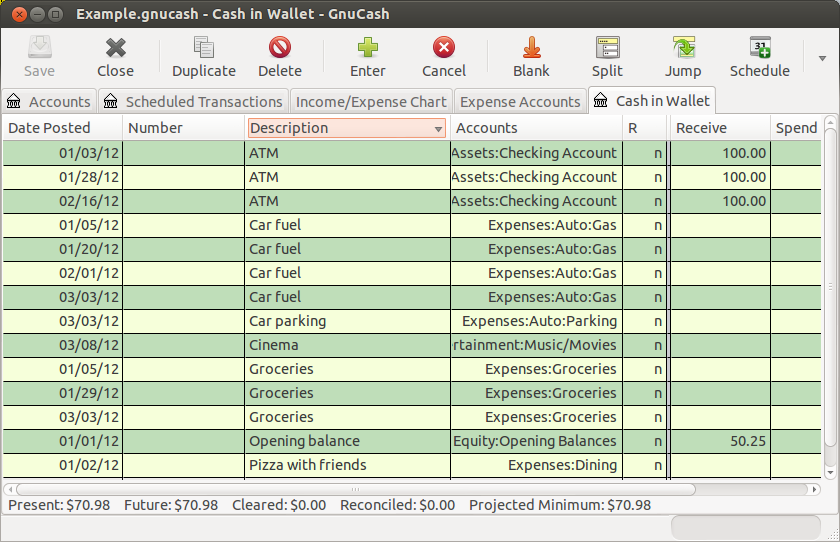
\includegraphics[width=\textwidth]{images/gnucash.png}
    \caption{Example GNU Cash UI \cite{GNUCashUI}}
    \label{fig:gnucash_ui}
\end{figure}

The main weakness of software like this is requiring users to import their data manually. Most users do not have all their accounts and transactions readily available in a structured format, and this is even worse when the user would want it to update live with their recent transactions. Few aspects of these applications help improve financial literacy, so few will be used in the final web application.

\subsection{Mobile Banking Applications}
\label{sec:mobile-banking-applications}
The next category is mobile banking applications. These are the default applications that come with each bank. Almost always, if the bank offers a website for online banking, they also offer a mobile application that performs the same functions. Examples include the major banks such as HSBC, NatWest, Lloyds, and online-only banks such as Monzo and Revolut. Often, these applications do not use open banking; instead, they work with the accounts from that specific company. Some do connect with other banks; however, they often do not incorporate these accounts into the analytics and instead, just display the balances.

Taking Revolut \cite{RevolutWebsite} as a case study, we can find its strengths to incorporate, as well as its weaknesses to avoid in the web application. Firstly, to even use Revolut's app functionality, users must open a bank account with the service and prove their identity. Although this gives the user confidence that their information is secure and personalised, it is also more challenging to use, slower to access the information, and overall is a catch. It also means that the app's primary purpose is not to provide a user with an overview of their finances but to provide a banking service, meaning it is not entirely focused on improving financial capability.

% \subsubsection{Strengths}
Some features of Revolut are worth acknowledging, such as the UI and ability to track expenditures. A slick and intuitive user interface enables users to understand all aspects of their finances and helps build confidence. In addition, expenditure tracking is beneficial, as it allows users to customise a budget for a set period and shows what and when they have spent money during this period; overall, aiming to help them stay within the budget.

% \subsubsection{Conclusion}
Revolut is a service that utilises open banking as it allows users to connect the app to their other bank accounts; however, it does not incorporate these into the budgets and only includes them in the net worth section. Revolut is an excellent example of a service that does use open banking but does not utilise it to its full potential.

\subsection{Paid Applications}
\label{sec:paid-applications}
The final category of applications is just the 'other' section; however, most of these incur costs to use. These applications are often more powerful than the free alternatives, yet are often filled with advertisements and are not as user-friendly. An excellent example is Quicken which won the awards for the best budgeting app in 2020 and 2021 \cite{Quicken}, but costs up to \textsterling 10 per month.

Quicken utilises open banking effectively to work with many different bank accounts, yet it does not enable quick-toggling of bank accounts to incorporate/ignore during the analysis and overview. This quick-toggling is a feature which would be particularly useful in giving better analytics, as a user would be able to segment all their savings accounts.

Despite having some useful budgeting features, Quicken cannot perform budgeting prediction from patterns in expenditure. This feature also would help improve financial capability because it will help the user plan for future expenses and identify areas where they can save money.

Overall, these paid applications have some aspects which would be helpful in the web application. However, they also are missing some basic ones, which would be more focused on improving financial literacy.

\section{Open Banking}
\label{sec:open-banking}
Open banking is defined as ``APIs [that] enable third-party developers to build applications and services around the financial institution'' in this paper \cite{OpenBankingDefinition}. Therefore, the open banking movement is the recent pressure on banks to open their data to third-party developers. They do this by creating a set of endpoints, which developers can design websites to query, and will respond with accurate and live data.

Each bank has its own set of endpoints, such that the authentication process and available information differ. Reading the documentation for each bank is time-consuming and not straightforward, yet learning how to interact with each bank's API is necessary to build an application that works with them all. This lack of standardisation is where Plaid \cite{Plaid} comes in.

\section{Plaid}
\label{sec:plaid}
Plaid is a platform that effectively wraps all the endpoints provided by the individual banks and provides a single standardised set of REST API endpoints as URLs. Using Plaid allows a third-party application only to query Plaid and, in turn, can support all the banks that Plaid provides access to - over twelve-thousand institutions \cite{PlaidInstitutions}.

\subsection{Plaid Tokens}
A strict authentication flow must be followed to use Plaid's endpoints because it handles private data. Plaid has three different types of tokens as part of this flow. The first is the link token.

Link is the widget's name and pop-up used to authenticate the user with their bank. To start this process requires a link token. These can be requested from Plaid's API and are valid for 4 hours, but are not tied to any user and do not treated like passwords.

Secondly, there are public tokens. These are what the link widget returns to the web application after the user has authenticated with their bank. They are unique to that user and are not treated like passwords, as they are valid for only 30 minutes and cannot be used to access a user's private information directly. In addition, they must be exchanged for an access token, the third type of token.

Exchanging the public token for an access token is done via a Plaid endpoint. However, because the access token must be treated like a password and be kept exceptionally securely, it is done via the web application's server rather than the client. If it is done on the client, it risks being exposed, and anyone with this token can access that user's information. Finally, a set of bank accounts can be embedded within the access tokens, and a user may have several associated access tokens.

\subsection{Plaid Authentication Flow}
\label{sec:plaid-authentication-flow}
The authentication flow used when interacting with Plaid is a strict process designed by the developer. It is described here, rather than in the design section, because it formed the foundation of the web application, and it heavily influenced the rest of the application's design. It is as follows:

\begin{itemize}
    \item The client requests a link token on behalf of the user
    \item The response link token is then passed to the link widget
    \item The user signs into their bank on the link widget pop-up
    \item The link widget returns a public token
    \item The client passes this public token to the backend
    \item The backend exchanges the public token for an access token
    \item The access token is stored in the database
\end{itemize}

Then suppose the user wishes to access their transactions:

\begin{itemize}
    \item The client queries the server acting as a proxy
    \item The server identifies which user is asking for the information
    \item That user's access token(s) are retrieved from the database
    \item The server sends a request to Plaid with the attached access token(s)
    \item The Plaid response is then forwarded back to the client
    \item Finally The client displays the information to the user
\end{itemize}

This flow can be seen as a sequence diagram in the figure below (\ref{fig:plaid_auth_flow}).

\begin{figure}[H]
    \centering
    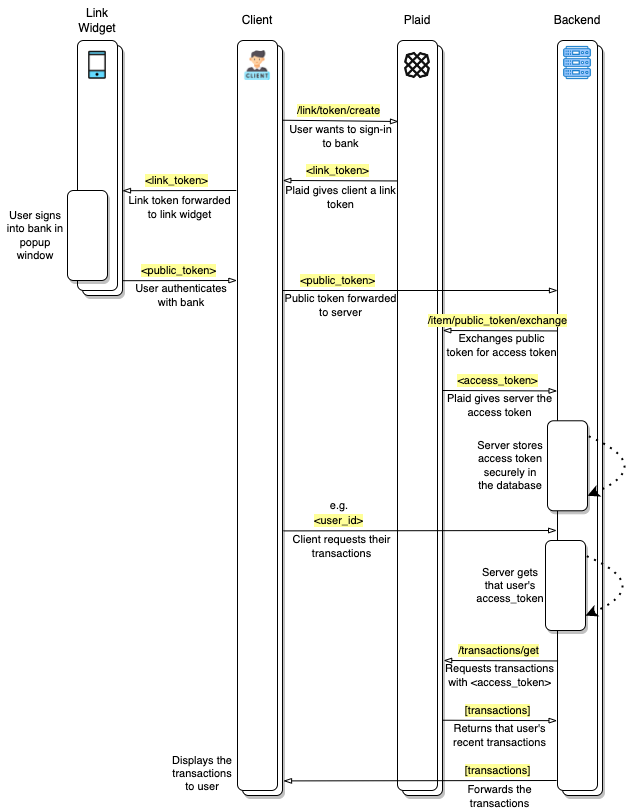
\includegraphics[width=\textwidth]{images/auth_flow_sequence_diagram.png}
    \caption{Plaid Authentication Flow Sequence Diagram}
    \label{fig:plaid_auth_flow}
\end{figure}

\subsection{Operation Modes}
\label{sec:plaid-operation-modes}
Further aspects of Plaid relevant to this project include the different modes of operation. When the web application queries Plaid's endpoints, one of three modes can be specified, each producing different results.

% \subsubsection{Sandbox Mode}
The first is sandbox mode which is the default. All the endpoints and request formats remain the same, but the responses are fake data generated by Plaid themselves. This mode helps test the web application without connecting to a bank, so do not worry about leaking any private information or getting fast and reliable responses.

% \subsubsection{Development Mode}
The second is development mode, where the responses are real data. The entire authentication flow must be followed in this mode, and a user will log in to their bank. To gain access to this mode, it must be requested from Plaid, and they review the application to ensure it is secure and will not leak any information. Once given access, there is a limit of one-hundred user accounts connected to actual banks, so this had to be managed carefully.

% \subsubsection{Production Mode}
The final mode is production mode. It is the same as development mode but with no limits. Further vetting is required to access this, and the queries now cost. For this project, only sandbox mode was initially used, and then following the completion of the prototype, development mode was requested and given for further testing and demonstrations.

\section{Further Motivation}
\label{sec:further-motivation}
As previously mentioned, the primary motivation for this project came from the recent open banking movement, so using modern technology to help push the field. In addition, the currently limited services available were also a factor, as it was identified that there was a need for an application like this. Finally, the timing for this project is very appropriate as the UK government announced that there is a financial crisis currently going on, which they named the 'Cost of Living Crisis' \cite{CostOfLivingCrisisGov}.

The Money and Pensions Service's recent report advised that people get a budget planner to help cope with the current times \cite{MaPS}. They are the government-sponsored financial guidance entity for the UK. The report helped concrete an objective for the web application to include budgeting features and would also help improve financial capability.